\documentclass{beamer}
\mode<presentation> {\usetheme{default}}
%\setbeamersize{text margin left=10mm,text margin right=10mm}


\setbeamertemplate{footline}[frame number]

\usepackage{amssymb}
\usepackage{amsthm}
\usepackage{amsmath}
\usepackage{booktabs}
\usepackage{needspace}
\usepackage{comment}
\usepackage{tikz}
\usepackage{graphicx}
\usepackage{bbm, dsfont}
\usepackage{array}
\usepackage{pgfplots}
\pgfplotsset{compat=1.16}

\usetikzlibrary{arrows,shapes,calc,positioning}

\theoremstyle{plain}
\newtheorem{thm}{Theorem}[section]
\newtheorem{cor}[thm]{Corollary}
\newtheorem{lem}[thm]{Lemma}
\newtheorem{prop}[thm]{Proposition}
%
\theoremstyle{definition}
\newtheorem{defn}{Definition}[section]
\newtheorem{remk}{Definition}[section]
\newtheorem{exam}{Example}[section]
\newtheorem{prob}{Exercise}[section]
\newtheorem{solu2}{Solution}[section]
\newenvironment{Shaded}{\begin{snugshade}}{\end{snugshade}}

\newcommand{\dif}{\operatorname{d}}
\newcommand{\var}{\operatorname{Var}}
\newcommand{\blue}[1]{\textcolor{blue}{#1}}
\newcommand{\purple}[1]{\textcolor{purple}{#1}}
\newcommand{\green}[1]{\textcolor{green!50!black}{#1}}

% Sections of Chapter 6 are numbered 6.1, 6.2, ...
\renewcommand{\thesection}{6.\arabic{section}}

% Annuity-immediate symbol: \ann{n}{i} gives a-angle-n at rate i
\newcommand{\ann}[2]{a_{\overline{#1|}#2}}

% Cash-flow timeline:
% \cfdiagram[extra tikz]{length}{tick position/label list}{position/amount list (above)}
\newcommand{\cfdiagram}[4][]{%
  \begin{tikzpicture}
    \draw (0,0) -- (#2,0);
    \foreach \x/\lab in {#3} {
      \draw (\x,0.12) -- (\x,-0.12);
      \node[below] at (\x,-0.12) {\scriptsize $\lab$};
    }
    \foreach \x/\amt in {#4} {
      \node[above] at (\x,0.12) {\scriptsize \amt};
    }
    #1
  \end{tikzpicture}%
}

% Blank for "F = ...  C = ..." rows
\newcommand{\blank}{\hspace{1.2cm}}

%opening

\title{RISK 201: Bonds}
\author{Himchan Jeong, FSA}
\institute{Department of Statistics \& Actuarial Science \\Simon Fraser University}
\date{}

\begin{document}
\maketitle

%======================================================================
\section{Introduction and terminology}
%======================================================================

\begin{frame}{6.1 Introduction and terminology}

\begin{itemize}
\item Bonds are financial instruments that corporations and governments use to raise capital
\item They are debt instruments:
  \begin{itemize}
  \item The \green{bond issuer} is the borrower: gets cash at issue, and will pay back principal and interest
  \item The \purple{bondholder} (investor) is the lender
  \end{itemize}
\item If the bond issuer does not make a payment as scheduled, we say they \textcolor{red}{defaulted} on the bond
\item Bonds are rated based on their probability of default
\end{itemize}

\end{frame}

\begin{frame}{Bond ratings}

\begin{center}
\renewcommand{\arraystretch}{1.2}
\small
\begin{tabular}{cccc}
\toprule
\multicolumn{2}{c}{\textbf{Bond Rating}} & & \\
\cmidrule(r){1-2}
\textbf{Moody's} & \textbf{Standard \& Poor's} & \textbf{Grade} & \textbf{Risk} \\
\midrule
Aaa & AAA & Investment & Lowest Risk \\
Aa & AA & Investment & Low Risk \\
A & A & Investment & Low Risk \\
Baa & BBB & Investment & Medium Risk \\
Ba, B & BB, B & Junk & High Risk \\
Caa/Ca/C & CCC/CC/C & Junk & Highest Risk \\
C & D & Junk & In Default \\
\bottomrule
\end{tabular}

\medskip
{\tiny Source: Investopedia (image by Sabrina Jiang \copyright\ Investopedia 2020)}
\end{center}

\end{frame}

\begin{frame}{Types of government bonds}

\begin{itemize}
\item \textbf{Savings bonds}: \purple{redeemable any time} (issuer will take it back and pay principal plus interest)
\item \textbf{Marketable bonds}:
  \begin{itemize}
  \item Have a specific \purple{maturity date}
  \item Usually not redeemable before maturity
  \item Bondholder can sell it to another investor
  \item Market price will depend on the characteristics of the bond as well as market conditions at time of sale
  \end{itemize}
\end{itemize}

\end{frame}

\begin{frame}{Terminology}

\renewcommand{\arraystretch}{1.3}
\small
\begin{tabular}{>{\raggedright\arraybackslash}p{0.26\textwidth}>{\raggedright\arraybackslash}p{0.66\textwidth}}
\toprule
Face value (par value) & Amount noted on front (face) of bond. Usually multiples of 100. \\
Maturity date & The date on which the loan is (normally) repaid. \\
Callable bond & A bond that can be redeemed before maturity at the discretion of the bond issuer, at specific dates, for specific amounts \\
Redemption date & A date on which the loan can be repaid \\
Redemption value & Amount payable at redemption date. ``At par'' means at face value. \\
\bottomrule
\end{tabular}

\end{frame}

\begin{frame}{Terminology, continued}

\renewcommand{\arraystretch}{1.3}
\small
\begin{tabular}{>{\raggedright\arraybackslash}p{0.26\textwidth}>{\raggedright\arraybackslash}p{0.66\textwidth}}
\toprule
Coupon rate (bond rate) & The rate at which the bond pays interest on its face value until the maturity date. Coupon payments are made at equal intervals (usually semiannually). \\
Yield rate (investment rate) & The rate of return realized by the bondholder on its investment. \\
\bottomrule
\end{tabular}

\end{frame}

\begin{frame}{Notation}

\renewcommand{\arraystretch}{1.3}
\begin{tabular}{r>{\raggedright\arraybackslash}p{0.8\textwidth}}
$F$: & face value \\
$C$: & redemption value \\
$r$: & coupon rate per interest period \\
$i$: & yield rate per interest period \\
$n$: & number of interest periods until maturity date \\
$P$: & purchase price of the bond \\
$Fr$: & coupon payment, received at the end of each interest period \\
\end{tabular}

\end{frame}

\begin{frame}{``Yield''}

\begin{itemize}
\item In practice, the coupon rate and the yield are quoted as nominal rates convertible semi-annually. For example, a ``5\% coupon bond yielding 8\%'' has $r = \blank$ and $i = \blank$.
\item Unless stated otherwise, the ``yield'' we will be calculating is the yield to maturity (YTM).
\item If the bond is sold before maturity, the investor may realize a different yield.
\end{itemize}

\end{frame}

%======================================================================
\section{Purchase price of a bond}
%======================================================================

\begin{frame}{6.2 Purchase price of a bond}

\begin{itemize}
\item Assumptions:
  \begin{itemize}
  \item No default
  \item Fixed maturity date
  \end{itemize}
\item Price is the present value of future payments (coupons plus redemption value)
\end{itemize}

\begin{center}
\cfdiagram[{\node[below] at (3,-0.12) {\scriptsize $\ldots$}; \node[above] at (3,0.12) {\scriptsize $\ldots$};}]
  {6}{0/0, 1/1, 2/2, 4/n-1, 5.5/n}{1/$Fr$, 2/$Fr$, 4/$Fr$, 5.5/$Fr+C$}
\end{center}

\[
P = Fr\,\ann{n}{i} + Cv^n
\]

\end{frame}

\begin{frame}{Example 6.1}

A \$1000 face value bond with 6\% coupons is redeemable at \$1200 at the end of 5 years.

\medskip
(a) What is the purchase price that yields 5\%?

\medskip
$F = \blank \quad C = \blank \quad n = \blank \quad r = \blank \quad i = $

\begin{center}
\cfdiagram{6}{0/0, 1/1, 2/2, 6/}{}
\end{center}

$P =$

\vfill
\end{frame}

\begin{frame}{Example 6.1, continued}

(b) What is the purchase price that yields 8\%?

\medskip
$F = \blank \quad C = \blank \quad n = \blank \quad r = \blank \quad i = $

\begin{center}
\cfdiagram{6}{0/0, 1/1, 2/2, 6/}{}
\end{center}

$P =$

\vfill
\end{frame}

\begin{frame}{Example 6.1, continued}

(c) What is the purchase price that yields 4\%?

\medskip
$F = \blank \quad C = \blank \quad n = \blank \quad r = \blank \quad i = $

\begin{center}
\cfdiagram{6}{0/0, 1/1, 2/2, 6/}{}
\end{center}

$P =$

\vfill
\end{frame}

\begin{frame}{Premium/discount formula}

An alternative formula for the price of a bond

\begin{center}
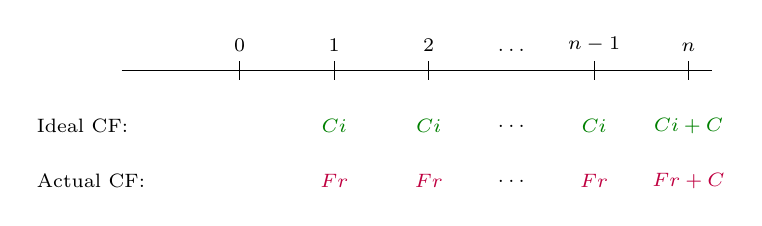
\begin{tikzpicture}
  \draw (0,0) -- (7.5,0);
  \foreach \x/\lab in {1.5/0, 2.7/1, 3.9/2, 6/n-1, 7.2/n} {
    \draw (\x,0.12) -- (\x,-0.12);
    \node[above] at (\x,0.12) {\scriptsize $\lab$};
  }
  \node[above] at (4.95,0.12) {\scriptsize $\ldots$};
  \node[anchor=west] at (-1.2,-0.7) {\scriptsize Ideal CF:};
  \node[anchor=west] at (-1.2,-1.4) {\scriptsize Actual CF:};
  \foreach \x/\amt in {2.7/Ci, 3.9/Ci, 6/Ci, 7.2/Ci+C} {
    \node at (\x,-0.7) {\scriptsize \green{$\amt$}};
  }
  \foreach \x/\amt in {2.7/Fr, 3.9/Fr, 6/Fr, 7.2/Fr+C} {
    \node at (\x,-1.4) {\scriptsize \purple{$\amt$}};
  }
  \node at (4.95,-0.7) {\scriptsize $\ldots$};
  \node at (4.95,-1.4) {\scriptsize $\ldots$};
\end{tikzpicture}
\end{center}

\[
P = C + (\purple{Fr} - \green{Ci})\,\ann{n}{i}
\]

\end{frame}

\begin{frame}{Example 6.1, continued}

Confirm the prices calculated earlier using the premium/discount formula

\medskip
\begin{center}
$F = \blank \quad C = \blank \quad n = \blank \quad r = \blank$
\end{center}

(a) $i = 2.5\%$

\vfill
(b) $i = 4\%$

\vfill
(c) $i = 2\%$

\vfill
\end{frame}

\begin{frame}{Auction process for GoC bonds}

\begin{itemize}
\item Gov't decides on face amount, term, coupon rate
\item Invites bids from investors for the yield they are willing to accept (to 3 decimals), and the amount of face value they are willing to buy
\item Yield is converted to price (5 decimals accuracy)
\item ``First price sealed bid'' auction:
  \begin{itemize}
  \item bids ranked from lowest to highest in terms of yield
  \item bids accepted in rank-order until desired amount is raised
  \item bids lower than threshold not accepted
  \item all accepted bids get the yield they proposed
  \end{itemize}
\end{itemize}

\end{frame}

\begin{frame}{Auction process, continued}

\begin{itemize}
\item Different from Dutch auction
\item Who can bid, and for what quantity, is limited
\item Competitive vs.\ non-competitive bids
\end{itemize}

\bigskip
\underline{Notes:}
\begin{itemize}
\item Process for issuing corporate bonds is different
\item After issue, bonds are traded in a dealer resale market
\end{itemize}

\end{frame}

%======================================================================
\section{Premium and Discount}
%======================================================================

\begin{frame}{6.3 Premium and Discount}

\begin{itemize}
\item Recall that a bond is essentially a loan from the investor to the bond issuer.
  \begin{itemize}
  \item The amount of the loan is the purchase price $P$
  \item The periodic payments $Fr$ together with the redemption value $C$ are enough to pay back the loan at interest rate $i$ per period
  \end{itemize}
\item We can draw up an amortization schedule for this loan, just like in Chapter 5
\end{itemize}

\end{frame}

\begin{frame}{Example 6.2}

Consider a \$1000 face value bond with 6\% coupons, redeemable for \$1200 at the end of 2 years, yielding 5\%.

\begin{center}
\begin{tikzpicture}
  \draw (0,0) -- (6,0);
  \foreach \x/\lab in {0/0, 1.5/1, 3/2, 4.5/3, 6/4} {
    \draw (\x,0.12) -- (\x,-0.12);
    \node[below] at (\x,-0.12) {\scriptsize $\lab$};
  }
  \foreach \x/\amt in {1.5/Fr, 3/Fr, 4.5/Fr, 6/Fr+C} {
    \node at (\x,-0.8) {\scriptsize \purple{$\amt$}};
  }
\end{tikzpicture}
\end{center}

\[
P = C + (\purple{Fr} - \green{Ci})\,\ann{n}{i} =
\]

\vfill
\end{frame}

\begin{frame}{Example 6.2, continued}

\begin{center}
\renewcommand{\arraystretch}{1.35}
\small
\begin{tabular}{cccc>{\centering\arraybackslash}p{0.17\textwidth}}
\toprule
\textbf{Period} & \textbf{Payment} & \textbf{Interest (at $i$)} & \textbf{Principal} & \textbf{Outstanding balance} \\
\midrule
0 & & & & 1,200 \\
1 & 30 & & & \\
2 & 30 & & & \\
3 & 30 & & & \\
4 & 30 & & & \\
4 & 1,200 & & & \\
\bottomrule
\end{tabular}
\end{center}

\end{frame}

\begin{frame}{Observations}

\begin{itemize}
\item When $P = C$, the coupon payments ($Fr$) exactly cover the interest accruing each period and no principal is paid back until maturity.
\item The outstanding balance on the loan is known as the \purple{book value} of the bond.
\item The book value immediately after a coupon payment can be calculated as the PV of the remaining payments (coupons plus redemption value) at rate $i$ per period. You can use either pricing formula to find this value.
\end{itemize}

\end{frame}

\begin{frame}{Example 6.3}

Consider a \$1000 face value bond with 6\% coupons, redeemable for \$1200 at the end of 2 years, yielding 3.1\%.

\begin{center}
\cfdiagram[{\foreach \x/\amt in {1.5/30, 3/30, 4.5/30, 6/{1,230}} {\node at (\x,-0.8) {\scriptsize \amt};}}]
  {6}{0/0, 1.5/1, 3/2, 4.5/3, 6/4}{}
\end{center}

\[
P = C + (Fr - Ci)\,\ann{n}{i} = 1{,}243.89
\]

$P > C$ we say the bond is \purple{purchased at a premium}

\end{frame}

\begin{frame}{Example 6.3, continued}

\begin{center}
\renewcommand{\arraystretch}{1.35}
\small
\begin{tabular}{cc>{\centering\arraybackslash}p{0.2\textwidth}c>{\centering\arraybackslash}p{0.17\textwidth}}
\toprule
\textbf{Period} & \textbf{Payment} & \textbf{Interest (1.55\% per period)} & \textbf{Principal} & \textbf{Outstanding balance} \\
\midrule
0 & & & & 1,243.89 \\
1 & 30.00 & & & \\
2 & 30.00 & & & \\
3 & 30.00 & & & \\
4 & 30.00 & & & \\
4 & 1,200.00 & & & \\
\bottomrule
\end{tabular}
\end{center}

\end{frame}

\begin{frame}{Observations ($P > C$)}

\begin{itemize}
\item When $P > C$, a portion of each coupon ($Fr$) goes towards repaying principal.
\item For a bond purchased at a premium, the \green{book value} gradually decreases from $P$ at time 0 to $C$ just after the last coupon payment. We say the book value is being \purple{written down}, or the \purple{premium is amortized}.
\item The \purple{amortization of the premium} in each coupon payment is the principal repayment portion.
\item Successive book value adjustments are in \purple{ratio $1+i$}.
\item The total amortization of premium is $P - C$.
\end{itemize}

\end{frame}

\begin{frame}{Example 6.4}

Consider a \$1000 face value bond with 6\% coupons, redeemable for \$1200 at the end of 2 years, yielding 8\%.

\begin{center}
\cfdiagram[{\foreach \x/\amt in {1.5/30, 3/30, 4.5/30, 6/{1,230}} {\node at (\x,-0.8) {\scriptsize \amt};}}]
  {6}{0/0, 1.5/1, 3/2, 4.5/3, 6/4}{}
\end{center}

\[
P = C + (Fr - Ci)\,\ann{n}{i} = 1{,}134.66
\]

$P < C$ we say the bond is \purple{purchased at a discount}

\end{frame}

\begin{frame}{Example 6.4, continued}

\begin{center}
\renewcommand{\arraystretch}{1.35}
\small
\begin{tabular}{ccccc}
\toprule
\textbf{Period} & \textbf{Payment} & \textbf{Interest} & \textbf{Principal} & \textbf{Outstanding} \\
 & & \textbf{(4\% per period)} & & \textbf{balance} \\
\midrule
0 & & & & 1,134.66 \\
1 & 30.00 & 45.39 & $-15.39$ & 1,150.05 \\
2 & 30.00 & 46.00 & $-16.00$ & 1,166.05 \\
3 & 30.00 & 46.64 & $-16.64$ & 1,182.69 \\
4 & 30.00 & 47.31 & $-17.31$ & 1,200.00 \\
4 & 1,200.00 & & 1,200.00 & 0.00 \\
\bottomrule
\end{tabular}
\end{center}

\end{frame}

\begin{frame}{Observations ($P < C$)}

\begin{itemize}
\item When $P < C$, the coupons are not enough to cover the interest accruing each period so the \purple{book value increases} over the life of the bond. We say the book value is being \purple{written up}, or the \purple{discount is accumulated}.
\item The amount for \purple{accumulation of discount} in each coupon payment is the amount by which the principal increases.
\item Successive book value adjustments are in ratio $1+i$.
\item Total book value adjustment is $P - C$.
\end{itemize}

\end{frame}

\begin{frame}{Book value vs.\ market value}

\begin{itemize}
\item The \textbf{book value} of a bond is the present value of the remaining coupons plus $C$ at the yield rate ($i$) in effect at the time of purchase.
\item After purchase, the book value may not be the price for which the bond could actually be sold in the open market.
\item If the yield rates available in the market at a later date ($i_t$) are different from the rate $i$ available at the time of purchase, then the \textbf{market value} of the bond will be different from the book value.
\end{itemize}

\end{frame}

\begin{frame}{Example 6.5}

Consider the bond in Example 6.4 ($F = 1000$, $C = 1200$, $r = 3\%$, $i = 4\%$). The book value at the end of the first year is \$1,166.05.

\begin{center}
\cfdiagram{6}{0/0, 1.5/1, 3/2, 4.5/3, 6/4}{}
\end{center}

Find the \textbf{market value} at the end of the first year if the prevailing yield rate is 12\% convertible semi-annually.

\vfill
\end{frame}

\begin{frame}{Example 6.5, continued}

If the investor bought the bond for \$1,134.66 at issue and sold it at market value at the end of the first year, what is the realized yield over the 1-year holding period?

\begin{center}
\cfdiagram{6}{0/0, 1.5/1, 3/2, 4.5/3, 6/4}{}
\end{center}

\vfill
\end{frame}

%======================================================================
\section{Price between coupon dates}
%======================================================================

\begin{frame}{6.4 Price between coupon dates}

\begin{itemize}
\item Purchase price formulas from 6.2 only work when the bond is issued or immediately after a coupon payment, so the remaining coupons are equally spaced.
\item If a bond is purchased between coupon payment dates, we need to adjust the price.
\item The book value of the bond increases as we get closer to each coupon payment date, and then drops when the coupon is actually paid.
\end{itemize}

\end{frame}

\begin{frame}{Full price of a bond}

\begin{itemize}
\item The \textbf{full price of a bond} is the total value of all future payments as of the purchase date.
\item The full price includes all of the value of the next coupon payment
\item At a point in time that is a portion $0 < k < 1$ of the way between two coupon payment dates, the full price is
\[
P = P_0(1+i)^k
\]
\item At the coupon payment date, the full price drops to
\[
P_1 = P_0(1+i) - Fr
\]
\end{itemize}

\end{frame}

\begin{frame}{Evolution of full price}

\begin{center}
\begin{tikzpicture}[scale=1.1]
  \draw[thick,->] (0,0) -- (8,0);
  \draw[thick,->] (0,0) -- (0,3.6);
  \foreach \x in {1,2,3} {
    \draw[thick] (2.2*\x-0.6,0.1) -- (2.2*\x-0.6,-0.1);
    \node[below] at (2.2*\x-0.6,-0.1) {\scriptsize \x};
  }
  \foreach \x/\y in {0/2.6, 1.6/2.15, 3.8/1.7, 6/1.25} {
    \fill (\x,\y) circle (2.5pt);
  }
  \node[below] at (4,-0.45) {\small Time (coupon payment periods)};
  \node[rotate=90] at (-0.4,1.8) {\small Bond price};
\end{tikzpicture}
\end{center}

\end{frame}

%======================================================================
\setcounter{section}{5}
\section{Determining the yield rate}
%======================================================================

\begin{frame}{6.6 Determining the yield rate}

To determine the yield on a bond:
\begin{itemize}
\item Use a financial calculator
\item Use Excel (YIELD)
\item Use interpolation between integer values
  \begin{itemize}
  \item Needs a starting point
  \item Consider the ``method of averages'' which approximates the true yield
  \end{itemize}
\end{itemize}

\end{frame}

\begin{frame}{The method of averages}

\[
\text{Approximate yield} = \frac{\text{Average interest payment}}{\text{Average amount invested}}
\]

\bigskip
\[
\text{Average interest payment:} \quad \frac{n \cdot Fr + C - P}{n}
\]

\bigskip
\[
\text{Average amount invested:} \quad \frac{P + C}{2}
\]

\end{frame}

\begin{frame}{Example 6.7}

Consider a \$1000 face value bond with 6\% coupons, redeemable for \$1200 at the end of 10 years. If the bond sells for \$1054, what is the yield?

\begin{center}
\cfdiagram{6}{0/0, 1.5/1, 3/2, 4.5/3, 6/4}{}
\end{center}

\bigskip
Average interest:

\vfill
Average amount invested:

\vfill
Approximate yield:

\vfill
\end{frame}

%======================================================================
\section{Other types of bonds}
%======================================================================

\begin{frame}{6.7 Other types of bonds}

A \purple{\textbf{zero-coupon bond}} (aka zero)
\begin{itemize}
\item Makes no coupon payments
\item Pays the face value at maturity
\item Sold at a discount relative to face value
  \begin{itemize}
  \item Aka discount bond or pure discount bond
  \end{itemize}
\item Price is PV of face value, discounted at yield rate
\item Examples:
  \begin{itemize}
  \item T-bills (short term, maturity $<$ 1 year)
  \item T-notes (intermediate term, less than 5 years)
  \item Stripped bonds (longer term)
  \end{itemize}
\end{itemize}

\end{frame}

\begin{frame}{Stripped bonds}

\begin{itemize}
\item An investor could:
  \begin{itemize}
  \item Buy a regular bond with coupons
  \item Resell the coupon payments and the redemption value separately
  \end{itemize}
\item The ``redemption only'' part is known as a \purple{\textbf{strip bond}}
\item Coupon payments could be sold individually or in groups
\end{itemize}

\end{frame}

\begin{frame}{Stripped bonds, continued}

\begin{itemize}
\item In the US, the Separate Trading of Registered Interest and Principal of Securities (STRIPS) program started in 1985.
\item In Canada, Canadian Depository Services Ltd.\ (CDS) has been stripping bonds electronically since 1987.
\end{itemize}

\end{frame}

\begin{frame}{Observed US Treasury yields (Feb 21)}

\begin{center}
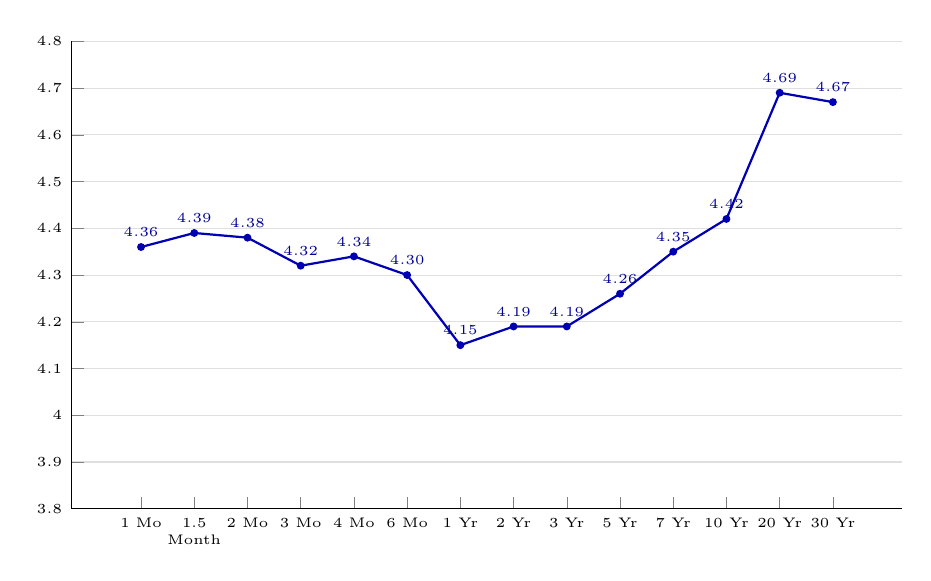
\begin{tikzpicture}
\begin{axis}[
  width=\textwidth, height=0.62\textwidth,
  ymin=3.8, ymax=4.8, ytick={3.8,3.9,...,4.81},
  yticklabel style={font=\tiny, /pgf/number format/fixed, /pgf/number format/precision=1},
  xtick={0,...,13},
  xticklabels={1 Mo, 1.5 Month, 2 Mo, 3 Mo, 4 Mo, 6 Mo, 1 Yr, 2 Yr, 3 Yr, 5 Yr, 7 Yr, 10 Yr, 20 Yr, 30 Yr},
  xticklabel style={font=\tiny, text width=0.7cm, align=center},
  ymajorgrids, grid style={gray!25},
  axis x line*=bottom, axis y line*=left,
  nodes near coords, nodes near coords style={font=\tiny, blue!60!black},
  every node near coord/.append style={/pgf/number format/fixed, /pgf/number format/precision=2, /pgf/number format/fixed zerofill},
]
\addplot[blue!70!black, thick, mark=*, mark size=1pt] coordinates {
  (0,4.36) (1,4.39) (2,4.38) (3,4.32) (4,4.34) (5,4.30) (6,4.15)
  (7,4.19) (8,4.19) (9,4.26) (10,4.35) (11,4.42) (12,4.69) (13,4.67)
};
\end{axis}
\end{tikzpicture}
\end{center}

\end{frame}

%======================================================================
\section{Callable Bonds}
%======================================================================

\begin{frame}{6.8 Callable Bonds}

\begin{itemize}
\item A callable bond is a bond which gives the \green{issuer} (not the \purple{bondholder}) the right to redeem prior to its maturity date, under certain conditions.
\item When issued, the \textbf{call provisions} explain when the bond can be redeemed and what the price will be.
\item In most cases, there is \textbf{some period of time} during which the \textbf{bond cannot be called}. This period of time is named the \textbf{call protection period}.
\end{itemize}

\end{frame}

\begin{frame}{Callable Bonds, continued}

\begin{itemize}
\item The earliest time to call the bond is named the \textbf{call date}.
\item The \textbf{call price} (could be different from the redemption value) is the amount of money the issuer must pay to buy the bond back.
\item Usually, bonds can be only called immediately after the payment of a coupon. If the bond is called immediately after the payment of $k$-th coupon, the present value of the obtained payments is
\[
P_k = C + (\purple{Fr} - \green{Ci})\,\ann{k}{i}
\]
\end{itemize}

\end{frame}

\begin{frame}{Callable bond pricing}

\begin{itemize}
\item $P_k$ is the price which the \purple{bondholder} would pay for the bond assuming that the bond is called immediately after the $k$-th coupon. The smaller $P_k$ is, the worse it is for the \purple{bondholder}.
\item Between all possible choices to recall a bond, the \green{issuer} will choose the option with the \textbf{smallest price}.
\end{itemize}

\end{frame}

\begin{frame}{Callable bond pricing}

\begin{itemize}
\item[(i)] if $\purple{Fr} > \green{Ci}$ (bond sells at a premium), $P_k$ increases with $k$, and we assume the \textbf{redemption date is the earliest possible}.
\item[(ii)] if $\purple{Fr} < \green{Ci}$ (bond sells at a discount), $P_k$ decreases with $k$, and we assume that the \textbf{redemption date is the latest possible}.
\item If a \purple{bondholder} wants to get an effective rate of interest of $i$ per period, then the maximum price which the \purple{bondholder} should pay is the lowest possible $P_k$ under that particular rate $i$.
\end{itemize}

\end{frame}

\begin{frame}{Example 6.6}

Consider a bond with $F = 100$, $r = 8\%$ with annual coupons callable at

\medskip
- 110 starting 10 years after issue for the next 5 year,

\medskip
- and maturing at 115 at the end of 15 years.

\medskip
What is the highest price which a \purple{bondholder} can pay and still be certain of an annual yield of 7\%?

\vfill
\end{frame}

\begin{frame}{Example 6.6, continued}

Case 1) If the bond is redeemed when $10 \le k < 15$:

\medskip
We have $C = 110$ and $Fr - Ci = 0.3 > 0$ so that the bond is sold at a premium (i.e., $P_k$ is increasing with $k$) so that it will be redeemed the earliest possible. Thus, the call price with Case 1 is
\[
P_{10} = 0.3\,\ann{10}{0.07} + 110 = 112.11.
\]

\end{frame}

\begin{frame}{Example 6.6, continued}

Case 2) If the bond is redeemed when $k = 15$:

\medskip
We have $C = 115$ and $Fr - Ci = -0.05 < 0$ so that the bond is sold at a discount (i.e., $P_k$ is decreasing with $k$) so that it will be redeemed the latest possible. Thus, the call price with Case 2 is
\[
P_{15} = -0.05\,\ann{15}{0.07} + 115 = 114.54.
\]

Therefore, the price of the callable bond is
\[
\min(112.11,\ 114.54) = 112.11.
\]

\end{frame}

\begin{frame}{SOA FM Samples}

{\footnotesize \url{https://www.soa.org/4a5549/globalassets/assets/files/edu/2018/2018-10-exam-fm-sample-questions.pdf}}

\medskip
72, 135, 136, 139, 142, 198, 292, 301, 378, 381

\end{frame}

\end{document}
